\section{rSLA implementation}\label{sec:runtime} 

rSLA is implemented as a DSL for cloud SLAs and the engine that supports their overall management aspects. As shown in Figure~\ref{fig:runtime}, rSLA engine provides support for the following loosely coupled SLA management operations: (1) SLA creation and activation, (2) monitoring and measurement of service metrics as specified in the SLA, (3) storage and processing of observed service metric values and of SLO evaluation results, (4) scheduling of rSLA objects to collect observations and evaluate SLOs according to their specified schedules, (5) service level evaluation and (6) notifications and reporting.
The next paragraphs highlight rSLA implementation aspects for all supported operations.

\subsection{SLA creation and activation}

As discussed in Section~\ref{language}, rSLA editing takes place using ruby programming blocks. The rSLA language exposes rSLA objects through code blocks that respect our DSL. When an rSLA runtime engine reads a new rSLA block, it generates an rSLA object that belongs to the block related class. 

To illustrate the creation and activation process of an SLA object in an rSLA runtime environment, we will assume that the context of Listings \ref{basescript} and \ref{sloscript} of Section \ref{language} represents the input that an rSLA service reads and processes. 

The attributes and function behavior of the generated object are mapped from the ruby block context to rSLA programming objects using the rSLA meta-interpretation programming library. Complete documentation on the rSLA language and currently implemented classes can be found at \cite{rSLAspec}.

On SLA object creation, an SLA can become active by triggering a schedule for the value measurement of the base metric or for the SLO evaluation. As soon as the scheduler service has set up measurement schedules for the new BaseMetric object or evaluation schedules for the SLO object, the SLA instance changes its state to \emph{ACTIVE}. 

\subsection{Monitoring and measurement}
Any SLA management framework requires a tool for monitoring and measuring metric values. For monitoring, rSLA engine currently uses a light weight mechanism called Xlets to handle the monitoring of base metric values. Section~\ref{sec:deployment} describes in detail the Xlets and their usage along with the deployment of rSLA as a compliance service in a cloud environment.

In rSLA service, the collection of monitoring observations are controlled by one or more schedules. Every base metric follows its own schedule. Afterwards, the measured metric observations are collected to a backend database for further processing. 
\subsection{Storage and processing}
Currently, rSLA is deployed on IBM Bluemix PaaS \cite{bluemix} and is configured to use Cloudant \cite{cloudant} database. Cloudant is a NoSQL database service provided by the PaaS. Based on the specified schedule, the values of base metrics are collected and stored as observation documents in the database. Cloudant uses map and reduce functions to collect and to efficiently process stored observations. 

Base metric value observations are required for the computation of composite metric values. Composite metrics specify aggregation functions between base as well as composite metric values that are needed to calculate their own values. Yet, base metric value observations can also be treated as time-series data and used for the creation of service level compliance analytics.

The persistence layer of rSLA is currently based on CouchRest \cite{couchrest} for the mapping of ruby objects to Cloudant documents. CouchRest uses REST HTTP requests to map rSLA object properties in 
the database. Associations between rSLA objects are described through the rSLA Cloudant data schema. Figure \ref{schema} illustrates  associations between rSLA objects in Cloudant.

Base, composite metrics as well as SLOs are associated with an SLA instance by a \textit{belongs to} relationship. Similarly, observations \textit{belong to} a base metric and evaluations and notifications data to an SLO. The \textit{belongs to} feature is defined in the CouchRest model as a property for the association of documents. It could be seen as an artificial foreign key to create associations between documents. 
\begin{figure}
\centering
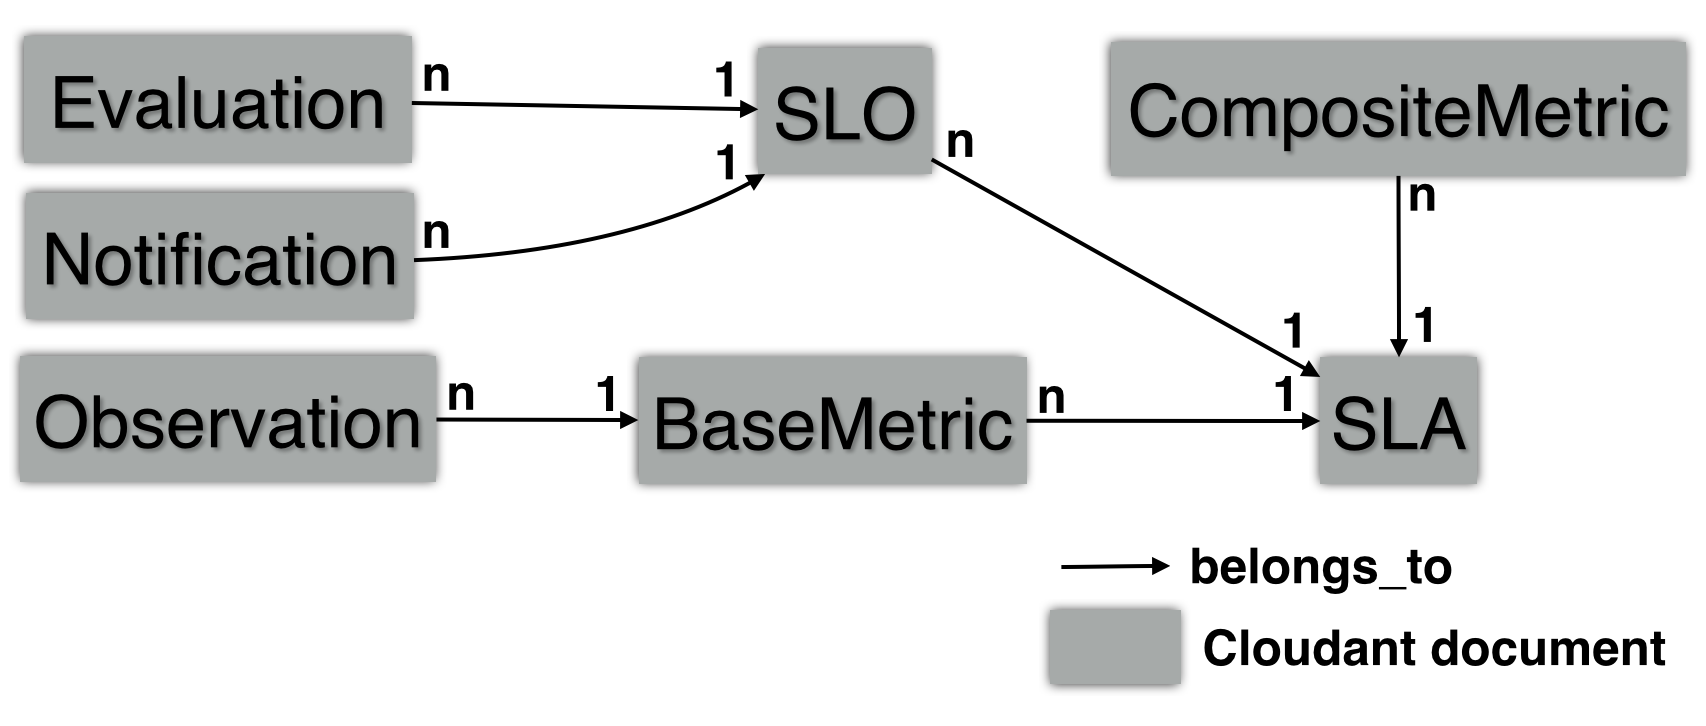
\includegraphics[width=0.5\textwidth]{pics/schema}
\caption{\label{schema} rSLA Cloudant object associations}
\end{figure}

Currently, processing of metric values may refers to compositions of base and/or composite metric values  for the creation of more aggregated composite metrics. The value computation of such metrics represents a computation that involves values of other metrics. Moreover, data value processing may refer to computations that are needed for the evaluation of one or more SLOs. Such computations may require input from data-value time-series to process the evaluation output.

%As discussed in Section \ref{sec:language}, expressions in rSLA denote free form statements that may take a conditional form or that may define data value computations.% The 
%computation for a composite metric value exemplifies an expression in rSLA. Composite metric values are used for the SLO evaluation. Expressions are used also for SLO evaluations 
%as preconditions 
%or objectives.

%Last but not least, the rSLA language library contains also a time series class that can be used for the application of statistical functions on time-series data sets. 

\subsection{Scheduling}\label{schedule}


When the rSLA engine receives a new SLA, it interprets this file to generate an SLA object in an \emph{INACTIVE} state. The inactive state indicates that 
the data collection of base metrics and the evaluation of SLOs are not yet associated to a scheduler. On SLA activation, the rSLA Service activates all base metrics and SLOs 
evaluation by sending their schedule description to the Scheduler. Consequently, the Scheduler associates a job for each of the base metrics and SLOs according to the specified 
scheduling data in the agreement. The Scheduler then starts triggering REST queries to activate the data collection for base metrics or evaluations for SLOs in a periodic manner. 

%In rSLA, composite metrics do not include a schedule because the computation of their values depends from SLO evaluation events. The SLO definition specifies a schedule for the 
%evaluation of precondition and objective expressions. Moreover, the evaluation of an SLO is accompanied with notification processes that send evaluation reports to the 
%customer/tenant.

The orchestration of scheduling events represents a topic of on-going work. Currently, rSLA uses the open source Rufus-scheduler that is an in-memory Ruby scheduler. We endowed 
this Scheduler with REST interfaces in order to allow decoupling it from the other parts of rSLA Service. These REST interfaces allow creating and deleting different types of 
recurrent jobs for base metrics and SLOs. 

\subsection{Service level evaluation and reporting}

Service level evaluation takes place at scheduled intervals. The frequency of service level evaluation is determined by schedule attributes in the SLO definition. As discussed in Section \ref{language}, the definition of an SLO encloses the expression of a precondition and of an objective. 
These two expressions follow sequential logic as illustrated by Listing \ref{precond} in Section \ref{language} to define the evaluation conditions that designate if the state of an SLO is healthy or not. These expressions use composite and base metric values to evaluate the SLO. The result of an SLO evaluation is a logical value ($true$ or $false$) that designates the service level objective state.

The evaluation process consists of the following steps: (1) parse the SLO expressions to fetch all required rSLA objects for their evaluation. (2) process such objects according to the expressions' statements. Such processing may involve fetching the values of base and/or composite and processing of such values, given some numerical function. (3) map the expression result output into its logical value and store the evaluation document.

The rSLA service level evaluation can be accompanied by a reporting step. This step consists of generating a notification based on the evaluation results. This notification contains a list of violations that occurred and the percentage of service levels that satisfied the objective target. Afterwards, this notification is sent to a reporting Xlet. This latter is endowed with a list of formatters that take as input a JSON document and generate a more readable format (e.g., CSV). The generated document is sent to a client to report the status of their provisioned resources. The reporting Xlet implements many protocols for reporting. Currently, we are using emails to send the reports to the clients. 

\subsection{Use-case pilot}

Currently, the rSLA service supports the management of cloud services that are leased by an existing customer. In one agreement, the IBM customer migrated a workload from a customer-owned, on-premise data center environment to the IBM cloud.  Along with the move, the customer required the monitoring of seven custom SLAs that had never been offered previously by the service provider in the cloud.

Each of the seven running SLAs consist of one base metric and of one service level objective. The rSLA service is running on the Bluemix platform and is aware of these seven agreements' context as such information is parsed by the rSLA engine to activate and initiate the measurement of involved base metrics. 

The rSLA service monitors, measures, evaluates and reports the service level status of the seven involved SLOs on a daily basis to the customer. Our reporting Xlet emails a daily notification report in CSV format.


